This chapter is dedicated to elaborate the design and the methodology of execution of the research project. The chapter commences with a thorough elaboration of the research methodology, followed by the detailed description of the sources of data which have been taken into consideration. Afterwards, the details of data collection strategy, data sanitisation and transformation strategy is described. Towards the conclusion of the chapter, the resultant data is summarised into appropriate visual forms of presentation.

\section{Computational Device as an Environment}

According to the \textit{Systems Thinking}, it is possible to portray the \textit{Computer} as a system. Typically a system,

\begin{itemize}
    \item has predefined objectives.
    \item has components interacting with each other.
    \item components cooperate and coordinate with each other to achieve the objectives.
    \item enclosed by a boundary.
    \item might or might not interact with the \textit{surrounding environment}.
\end{itemize}

An abstract schematic that graphically depicts this outline could be sketched as in figure \ref{fig:abs_sys}. It is quite straightforward that this approach enables identifying two distinct partitions of the space that the system exists. Those are namely,

\begin{itemize}
    \item \textit{Internal Environment} - The space that which is within the system's boundary
    \item \textit{External Environment} - The space that which is out of the system's boundary
\end{itemize}

\begin{figure}[h!]
    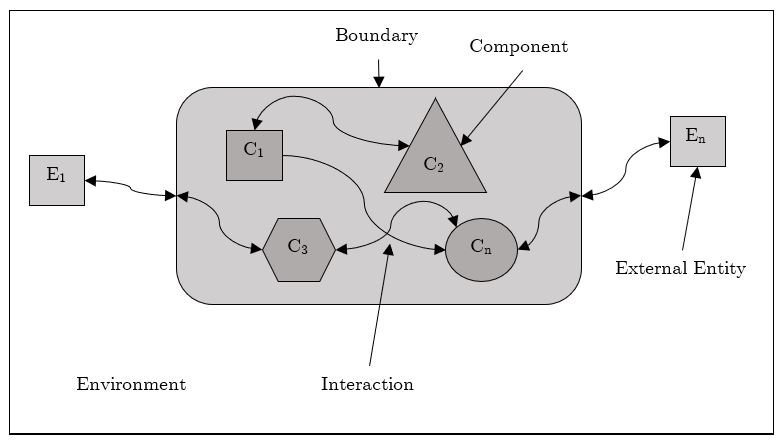
\includegraphics[width=0.6\textwidth]{system_schem.JPG}
    \centering
    \caption{Abstract Schematic of a System}
    \label{fig:abs_sys}
\end{figure}

This research identifies both of these partitions as \textit{the Environment}. The research focuses on the phenomenon that takes place in this environment. The observations made by the author along with the assumptions and interpretations are discussed in detail in the following chapter*****.

\section{Extraction and Visual Inspection}
Identifying different phenomenon from this environment of the computational device and collecting the metrics related to those are the activities which are due on the \textit{Extraction} phase. There, primarily the following sources were considered as data sources for extraction of randomness.

\begin{enumerate}
    \item Device metrics such as \acrfull{ram} usage, \acrfull{cpu} usage, temperature measures and so forth.
    \item Network packet flows. Here, it was mainly focused on the wireless network adapters that the device is having built in. Specifically the \acrfull{wlan} adapters that the device is having and operating in the \textbf{\textit{monitor mode}} (also known as \textbf{\textit{promiscuous mode}}) was extensively used.
\end{enumerate}

The reason behind choosing these sources was primarily due to the readily availability. One of the main motives behind this study is to discover the ability for an ordinary personal computational device to generate randomness while being portable, cost effective and performant. Costly peripherals attached to the devices via cables or any other source, would not be positively supporting to uphold that motive. Moreover, large volumes of systematic, structured and intentional data flows are quite effective in concealing subtle, less important yet useful effects which the causes are uncertain and unpredictable.

The data extracted from the sources were visually inspected in the second stage so as to filter out any obvious and frequently repeating data points and items. These data items would quite useful if the security of the application is not much of an importance. However, since this is intended to be useful in security critical applications as well, such frequent and obvious data needs to be filtered. That was decided to be done based on a visual inspection.

Even though the network traffic data was collected, they were not taken into consideration during the next steps due to the added complexity of reliability of those data, as those data are originated well away from the system boundary. However, these could be considered in expanding this study further.

\section{Distillation}

Distillation is the phase where the data points which sequentially together demonstrate absence of patterns, are extracted from the filtered sources. During the extraction of data, initially the collected data pool was visually inspected using small \textit{sliding windows}\footnote{A predetermined time frame of fixed length, that will be sled across a sequence from the beginning to the end. At any point in time, what belongs to within the time frame is taken into consideration} of time. The variation of each observed attribute across the sliding window was considered and the attributes which does not demonstrate rapid changes were dropped out. For the ease of observation, these data were tabulated and visually inspected over approximately 1000 samples. End result of the distillation would be microscopic data points/values, or macroscopic values which could be used to generate microscopic results with the use of  some operation or a combination of operations,  which will provide the seeds for transformation in the next step.

\section{Transformation}

During the transformation, the seeds from the previous stage are transformed into different representations in order to meet the volume and complexity requirements of the randomness. Since the requirement is a large bit string which is sufficiently complex, the primary alternative considered was \textit{Floating Point Number System}.

\subsection{Floating Point Representation System}
\textit{Floating Point Representation} is a binary representation of a fractional number, which is which is widely used in modern day computers. A Floating Point representation attempts to capture and represent the following details about the particular number.

\begin{enumerate}
    \item Sign (represented by $s$)
    \item Exponent (represented by $E$) - A measure of the position of the decimal point of the number being represented.
    \item Significand (also known as \textit{Mantissa}, represented by $m$) - The actual value of the number.
\end{enumerate}

Usually, to represent the sign, a single bit would be allocated. For the other two parameters there are standard value combinations as well as arbitrary settings. When a number is represented using floating point

\begin{enumerate}
    \item The number is represented in the binary number system.
    \item Binary number is normalised (discussed in subsection \ref{sec_norm_exp} below).
    \item The index of two (2) is obtained and transformed using the bias (discussed in subsection \ref{sec_norm_exp} below) and the biased exponent is converted to binary. This will be assigned to $E$.
    \item Fractional bits of the normalised number is assigned to $m$.
    \item $\text{CONCATENATE}(s, E, m)$ will be the final representation of the number.
\end{enumerate}

\subsection{Normalisation of the Binary Number and Exponent}\label{sec_norm_exp}

If the number $+13.25_{10}$ is taken into consideration for an instance, it's binary representation would be $+1101.01_2$. In applied mathematics, a number is said to be normalised when it is written in scientific notation with one non-zero decimal digit before the decimal point \cite{bk_math_of_astro}. So, the above number in decimal could be written as $+1.325 \times 10^1$. The same process on the binary representation would result in $+1.10101 \times 2^3$. It is also important to note that, if the first two steps are interchanged, the result would be drastically different.

As per the steps above, next is to convert the index of two to binary. Now if an imaginary result of a binary conversion of a fraction is considered such as $0.000101$, normalising such would result in $1.01 \times 2^{-4}$, which the index of two is a negative number. This causes another problem of representing signed magnitudes. This could in a way be overcome by representing this using a number representation such as \textit{2's complement}. However, since 2's complement would make the forward process and the reversal process too much complicated, and since this is not directly used in any arithmetic operations, it is possible to reliably use a \textit{bias value}, which would map an interval $\{-n \twodots n+1\}$ to an interval $\{0 \twodots 2n-1\}$. The bias value is based on the number of bits allocated as the exponent and for $i$ which is the number of bits in exponent, bias value is given by $2^i-1$.

\subsection{Analysis on Attributes of Floating Point}\label{subsec:float_attr}

Previously it has been established that floating point is an approximate representation of a fractional number. If the fractional number $3.2$ is considered for an instance, representing this as a binary number would result in $11.001100110011\twodots$. Upon closer examination, it is evident that the fractional part of the binary representation above, has a repetitive pattern of $\dot{0}01\dot{1}$. Apart from those special cases, many floating point representations were appearing to have an uneven spread of binary digits across the representation. So, it is decided to closely review the behaviour of floating point representations to identify its usability as a \textit{model of transformation} of certain metrics. This review was conducted according to the following routine.

\begin{enumerate}
    \item Implement a routine for floating point conversion of arbitrary structures.
    
    \item \label{lbl:mantissa} Starting from one digit at the mantissa in the decimal number, convert the given mantissa to binary. Here, the length of the mantissa $m$ was chosen to be around $10^6$. It could be extended beyond that however, such cases will be sensitive to the performance of the device being used.
    
    \item Once the bit string is generated, plot the bits into an $x \times y$ (where $x\cdot y=m$) bitmap for visualisation.
    
    \item At the end of each iteration, append a randomly chosen digit (here the digit is chosen by author with no conscious intervention) to the input on the previous stage, and repeat from step \ref{lbl:mantissa}.
\end{enumerate}

A separate routine that generates the bitmaps were implemented using Python with the use of \ilcode{matplotlib}. \ilcode{matplotlib} is a powerful module that could be plugged into Python, for a vast variety of image processing tasks. Once the above process is repeated for over 1000 times for different choices of digits, it was decided to visually and mathematically evaluate the bitmaps. Based on those, it is possible to discover the patterns and assess their closeness to randomness. For the benchmark of this activity, a bitmap which is captured from a television which was out of synchronisation with a visual signal, was used (Figure \ref{fig:radnbits_randomorg}) and each bitmap was compared visually, mathematically and then the data and the observations were tabulated.

\begin{figure}[h!]
    
\includegraphics[width=0.6\textwidth]{randbitmap_randomorg.png}
    \centering
    \caption{Television Noise generated, during absence of a Signal}
    \label{fig:radnbits_randomorg}
\end{figure}

Each bitmap generated above, were structurally compared using \acrfull{mse}. MSE is a measure of average of the squared errors for each pixel of the image. For each sample, the MSE is calculated and plotted in a graph, in order to evaluate the variation as the number of digits increased. A visual inspection on each image also was carried out in order to note the perceivable differences and variations. This test is hereafter identified by the name \textit{Initial Random String Test}.

\section{Hardening}\label{sec:hardening_details}

Hardening is an optional phase, which would only be required in the context of security critical applications such as cryptography. Intention of this phase is to make sure that the data being generated becomes more tamper proof. This stage is primarily essential to inculcate the attributes of a \textit{Cryptographically Secure Random Number Generator}, which in brief are

\begin{enumerate}
    \item Given that the first $k$ bits of a random sequence is known, there should not exist a polynomial time algorithm that would predict the $k+1^{\text{th}}$ bit, any better than 50\% of success.
    
    \item In case if a part of the sequence is successfully asserted, it should not be possible to predict the part of the sequence before the revelation.
    
    \item If the generator uses some sort of an entropy input, it is expected to be infeasible to utilise the knowledge on the state of the input for predicting future conditions of the generator.
\end{enumerate}

Specially, the \nth{3} point on the above list is crucial in a security critical application. In order to achieve this, following alternatives were taken into consideration.

\subsection{Symmetric vs. Asymmetric Key Encryption}

\textit{Symmetric Key Encryption} (also known as \textit{Private Key Encryption}) is one of the two fundamental flavours of data encryption. The absolute purpose of encryption is to hide the meaning of some message from everyone else except the intended recipients. This is primarily some function $E(m,k)$ where $m$ is the message and $k$ is the encryption key. The reason for this to be known as symmetric is that, to decrypt and reveal the original plain text, the same key that was for encryption is used, which is where the symmetry of the process is considered at.

\textit{Asymmetric Key Encryption} (also known as \textit{Public Key Encryption}) is the counterpart flavour of the previous. Popular and widely used encryption schemes such as RSA, ECC and so forth. Here also exists some function $F(m,K)$ where $m$ is the message and $K$ is the encryption/decryption key. Here, the asymmetry comes from the fact that the $K$ in fact are two interrelated keys $k_p$ and $k_u$ in such a way that, what is encrypted with $k_p$ could only be decrypted by $k_u$ and vice versa. This addresses certain inherent issues in symmetric key encryption such as key distribution problem. Since the two keys are entirely different, the term \textit{asymmetric} is coined. However, schemes of this model are having certain other drawbacks such as implementation complexity and specially, most of the encryption schemes of this family requires a random \acrfull{iv}, which causes a \textit{cyclic dependency} between random number generation and asymmetric encryption, for most of the algorithms.

Due to the obvious reasons it has been decided to lean towards symmetric encryption. This leaves the following concerns to be addressed when an encryption scheme is chosen.

\begin{enumerate}
    \item Resistant to attacks
    \item Less implementation complexity for being compatible with the personal computing devices
    \item Less consumption of computational power for being compatible with the personal computing devices
\end{enumerate}

As discussed previously in section \ref{subsec:aes}, AES has some powerful features which are quite useful along subtle weaknesses that could be overcome with caution. When AES works in CBC mode, it requires an IV, that which could be provided as a password for the system, which enables enforcing standards over the password. Since the encryption process does not require to have a decryption process, the administrator(s) will not have the requirement to remember the password, which will enable enforcing strict standards. This will provide the additional security required to meet the cryptographic security standards.

\subsection{Message Digest and Hashing}
\textit{Hashing}, which is also known widely as \textit{Message Digest} is a process of mathematically transforming an input of an arbitrary size, to an output which is most f the times of fixed size. Precisely, hash functions generate an output which is called the \textit{Message Digest}. Typical work flow of a hashing algorithm is as depicted below (Figure \ref{fig:wrk_flw_hash}).

\begin{figure}[h!]
    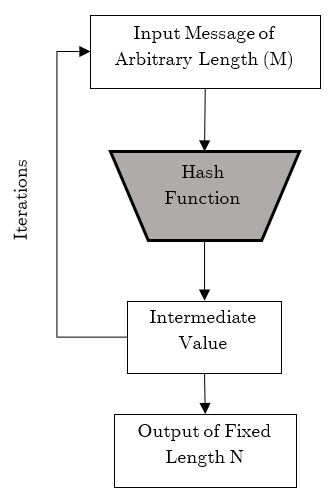
\includegraphics[width=0.5\textwidth]{hash_schem.JPG}
    \centering
    \caption{Work flow of a Hash Function}
    \label{fig:wrk_flw_hash}
\end{figure}

The most important attribute of hashing is that, given only the output it is a process which cannot be reversed to obtain the initial input or the state of the algorithm. This makes hashing a powerful function, which has attributes that could be leveraged in generating random numbers. There already are a wide variety of RNGs which are based on hashing algorithms. Such algorithms include but not limited to \textit{Hash\_DBRG, HMAC\_DBRG, CTR\_DBRG} and so forth \cite{rep_nist_sp_80090a}.

\subsection{Use of Hashing within the Context}
Hashing was considered as an option for hardening in the context of this research. Since hashing is an irreversible process, a block which appears to be arbitrary could be easily hidden by using hashing, as the reverse mapping is not present and computationally infeasible to generate that. However, all the available hashing algorithms are generating lengthy hashes (about 128 bits and above), which would bring in the requirement of clipping their outputs. This would add more overhead and dependencies on additional functions such as sponge functions\footnote{Finite state algorithms that take a bit stream of any length to produce a bit stream of a given length}. Hence hashing was left out from further consideration, as a possible further work.